\let\negmedspace\undefined
\let\negthickspace\undefined
%\RequirePackage{amsmath}
\documentclass[journal,12pt,twocolumn]{IEEEtran}
 \usepackage{gensymb}
%\doublespacing
 \usepackage{polynom}
 \usepackage{float}
%\singlespacing
%\usepackage{silence}
%Disable all warnings issued by latex starting with "You have..."
%\usepackage{graphicx}
\usepackage{amssymb}
%\usepackage{relsize}
\usepackage[cmex10]{amsmath}
\newcount\tmpnum
\def\tallymarks#1{\leavevmode \lower1bp\vbox to9bp{}%
   \tmpnum=#1
   \loop \ifnum\tmpnum<5 \kern1bp \tallynum\tmpnum \else \tallyV \fi
         \advance\tmpnum by-5
         \ifnum\tmpnum>0 \repeat
}
\def\tallynum#1{\bgroup\tmpnum=#1\relax
   \loop \ifnum\tmpnum>0
         \kern1bp \tallyI \kern1bp
         \advance\tmpnum by-1
         \repeat
   \egroup
}
\def\tallyI{\pdfliteral{q .5 w 0 -1 m 0 8 l S Q}}
\def\tallyV{\kern1bp\pdfliteral{q .5 w -1 0 m 9 7 l S Q}\tallynum4\kern1bp }

\usepackage{amsthm}
%\usepackage{pifont}
%\usepackage{iithtlc}
% \usepackage{mathrsfs}
% \usepackage{txfonts}
 \usepackage{stfloats}
% \usepackage{steinmetz}
 \usepackage{bm}
% \usepackage{cite}
% \usepackage{cases}
% \usepackage{subfig}
%\usepackage{xtab}
\usepackage{longtable}
%\usepackage{multirow}
%\usepackage{algorithm}
%\usepackage{algpseudocode}
\usepackage{enumitem}
 \usepackage{mathtools}
 \usepackage{tikz}
% \usepackage{circuitikz}
% \usepackage{verbatim}
%\usepackage{tfrupee}
\usepackage[breaklinks=true]{hyperref}
%\usepackage{stmaryrd}
%\usepackage{tkz-euclide} % loads  TikZ and tkz-base
%\usetkzobj{all}
\usepackage{listings}
    \usepackage{color}                                            %%
    \usepackage{array}                                            %%
    \usepackage{longtable}                                        %%
    \usepackage{calc}                                             %%
    \usepackage{multirow}                                         %%
    \usepackage{hhline}                                           %%
    \usepackage{ifthen}                                           %%
  %optionally (for landscape tables embedded in another document): %%
    \usepackage{lscape}     
% \usepackage{multicol}
% \usepackage{chngcntr}
%\usepackage{enumerate}
\usepackage{tfrupee}

%\usepackage{wasysym}
%\newcounter{MYtempeqncnt}
\DeclareMathOperator*{\Res}{Res}
\DeclareMathOperator*{\equals}{=}
%\renewcommand{\baselinestretch}{2}
%\renewcommand\thesection{\arabic{section}}
%\renewcommand\thesubsection{\thesection.\arabic{subsection}}
%\renewcommand\thesubsubsection{\thesubsection.\arabic{subsubsection}}

%\renewcommand\thesectiondis{\arabic{section}}
%\renewcommand\thesubsectiondis{\thesectiondis.\arabic{subsection}}
%\renewcommand\thesubsubsectiondis{\thesubsectiondis.\arabic{subsubsection}}

% correct bad hyphenation here
\hyphenation{op-tical net-works semi-conduc-tor}
\def\inputGnumericTable{}                                 %%

\lstset{
frame=single, 
breaklines=true,
columns=fullflexible
}
\newtheorem{theorem}{Theorem}[section]
\newtheorem{problem}{Problem}
\newtheorem{proposition}{Proposition}[section]
\newtheorem{lemma}{Lemma}[section]
\newtheorem{corollary}[theorem]{Corollary}
\newtheorem{example}{Example}[section]
\newtheorem{definition}[problem]{Definition}
%\newtheorem{thm}{Theorem}[section] 
%\newtheorem{defn}[thm]{Definition}
%\newtheorem{algorithm}{Algorithm}[section]
%\newtheorem{cor}{Corollary}
\newcommand{\BEQA}{\begin{eqnarray}}
\newcommand{\EEQA}{\end{eqnarray}}
\newcommand{\define}{\stackrel{\triangle}{=}}
\newcommand*\circled[1]{\tikz[baseline=(char.base)]{
    \node[shape=circle,draw,inner sep=2pt] (char) {#1};}}
\bibliographystyle{IEEEtran}
%\bibliographystyle{ieeetr}
\providecommand{\mbf}{\mathbf}
\providecommand{\pr}[1]{\ensuremath{\Pr\left(#1\right)}}
\providecommand{\qfunc}[1]{\ensuremath{Q\left(#1\right)}}
\providecommand{\sbrak}[1]{\ensuremath{{}\left[#1\right]}}
\providecommand{\lsbrak}[1]{\ensuremath{{}\left[#1\right.}}
\providecommand{\rsbrak}[1]{\ensuremath{{}\left.#1\right]}}
\providecommand{\brak}[1]{\ensuremath{\left(#1\right)}}
\providecommand{\lbrak}[1]{\ensuremath{\left(#1\right.}}
\providecommand{\rbrak}[1]{\ensuremath{\left.#1\right)}}
\providecommand{\cbrak}[1]{\ensuremath{\left\{#1\right\}}}
\providecommand{\lcbrak}[1]{\ensuremath{\left\{#1\right.}}
\providecommand{\rcbrak}[1]{\ensuremath{\left.#1\right\}}}
\theoremstyle{remark}
\newtheorem{rem}{Remark}
\newcommand{\sgn}{\mathop{\mathrm{sgn}}}
\providecommand{\fourier}{\overset{\mathcal{F}}{ \rightleftharpoons}}
%\providecommand{\hilbert}{\overset{\mathcal{H}}{ \rightleftharpoons}}
\providecommand{\system}{\overset{\mathcal{H}}{ \longleftrightarrow}}
	%\newcommand{\solution}[2]{\textbf{Solution:}{#1}}
\newcommand{\solution}{\noindent \textbf{Solution: }}
\newcommand{\cosec}{\,\text{cosec}\,}
\providecommand{\dec}[2]{\ensuremath{\overset{#1}{\underset{#2}{\gtrless}}}}
\newcommand{\myvec}[1]{\ensuremath{\begin{pmatrix}#1\end{pmatrix}}}
\newcommand{\mydet}[1]{\ensuremath{\begin{vmatrix}#1\end{vmatrix}}}
\makeatletter

\makeatother
\let\StandardTheFigure\thefigure
\let\vec\mathbf

\def\putbox#1#2#3{\makebox[0in][l]{\makebox[#1][l]{}\raisebox{\baselineskip}[0in][0in]{\raisebox{#2}[0in][0in]{#3}}}}
     \def\rightbox#1{\makebox[0in][r]{#1}}
     \def\centbox#1{\makebox[0in]{#1}}
     \def\topbox#1{\raisebox{-\baselineskip}[0in][0in]{#1}}
     \def\midbox#1{\raisebox{-0.5\baselineskip}[0in][0in]{#1}}
\title{Assignment 3}
\author{ Vedant Bhandare (cs21btech11007)}

\begin{document}

\maketitle
\begin{abstract}
This document contains the solution for Assignment 3 (CBSE Class 9 Chapter 14 (Probability) Example 3
\end{abstract}
\maketitle

\textbf{Example 3: } 100 plants each were planted in 100 schools during Van Mahotsav. After one month, the number of plants that survived were reccorded as :
\begin{center}
\begin{tabular}{c c c c c c c c c c}
95 & 67 & 28 & 32 & 65 & 65 & 69 & 33 & 98 & 96\\
76 & 42 & 32 & 38 & 42 & 40 & 40 & 69 & 95 & 92\\
75 & 83 & 76 & 83 & 85 & 62 & 37 & 65 & 63 & 42\\
89 & 65 & 73 & 81 & 49 & 52 & 64 & 76 & 83 & 92\\
93 & 68 & 52 & 79 & 81 & 83 & 59 & 82 & 75 & 82\\
86 & 90 & 44 & 62 & 31 & 36 & 38 & 42 & 39 & 83\\
87 & 56 & 88 & 23 & 35 & 76 & 83 & 85 & 30 & 68\\
69 & 83 & 86 & 43 & 45 & 39 & 83 & 75 & 66 & 83\\
92 & 75 & 89 & 66 & 91 & 27 & 88 & 89 & 93 & 42\\
53 & 69 & 90 & 55 & 66 & 49 & 52 & 83 & 34 & 36
\end{tabular}
\end{center}
\textit{Prepare a grouped frequency distribution table to represent the above raw data, and hence find class width and number of schools with more than 50\% plants survived.}\\
\\
\textbf{Solution: }
\begin{center}
\begin{tabular}{|c|c|c|}
\hline
Number of plants & Tally & Number of schools \\
survived & Marks & (frequency)\\
\hline
20 - 29 & \tallymarks{3} & 3\\
30 - 39 & \tallymarks{14} & 14\\
40 - 49 & \tallymarks{12} & 12\\
50 - 59 & \tallymarks{8} & 8\\
60 - 69 & \tallymarks{18} & 18\\
70 - 79 & \tallymarks{10} & 10\\
80 - 89 & \tallymarks{23} & 23\\
90 - 99 & \tallymarks{12} & 12\\
\hline
\end{tabular}
\end{center}
\begin{center}
TABLE 1: Group frequency distribution table
\end{center}
Class width = 10\\
Number of schools with more than 50\% plants survived = 8 + 18 + 10 + 23 + 12 = 71

\begin{figure}[H]
    \centering
    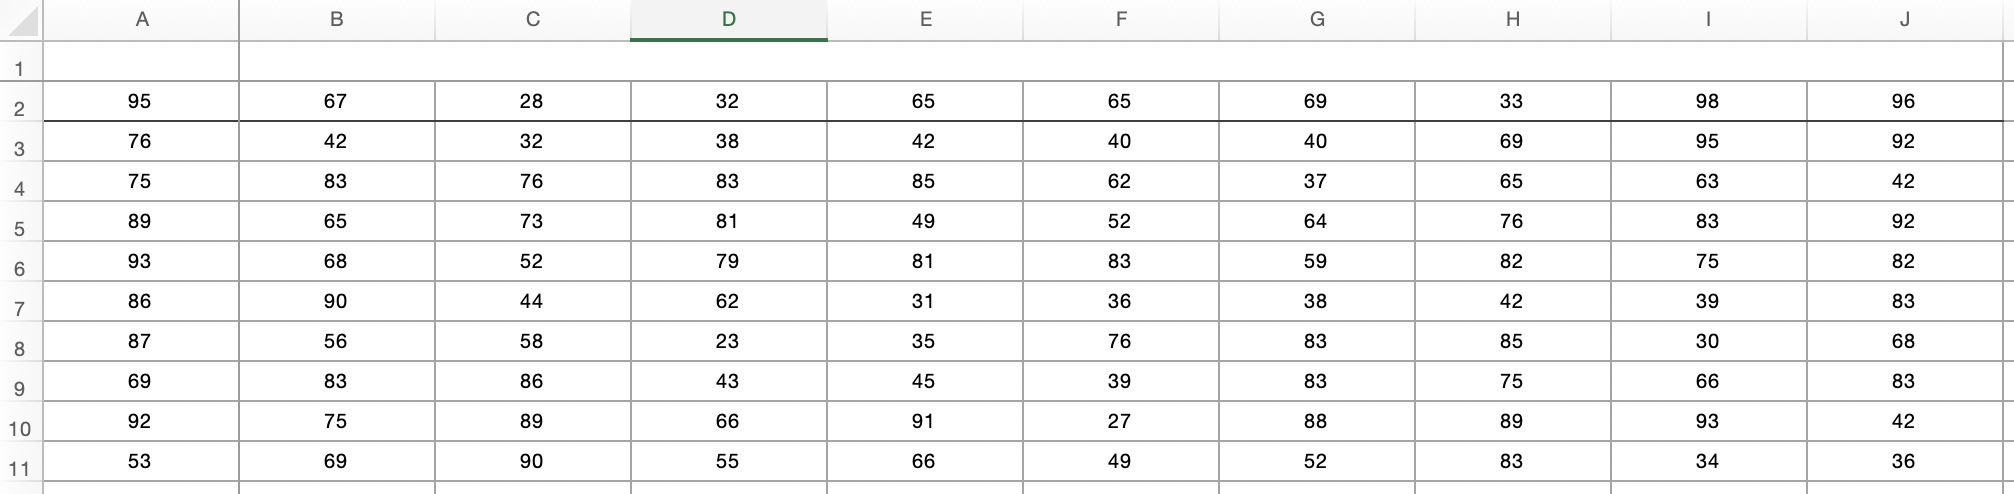
\includegraphics[width=\columnwidth]{ExcelFiles/raw_data.png}
    \caption{Python code reads from the rawdata.xlsx}
    \label{fig1}
\end{figure}
\begin{figure}[H]
    \centering
    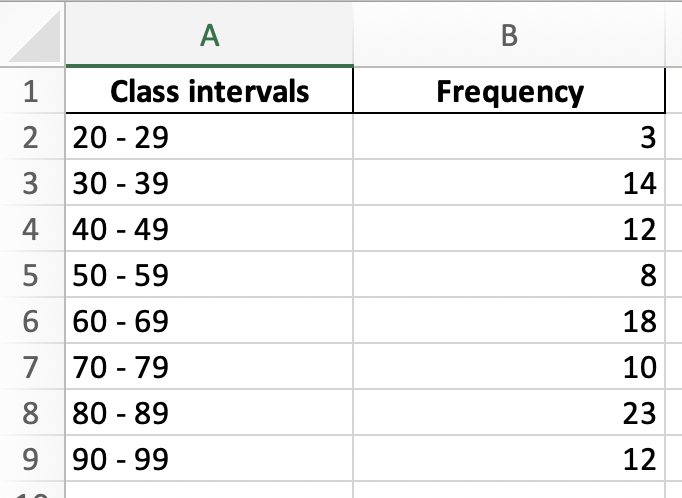
\includegraphics[width=\columnwidth - 4mm]{ExcelFiles/frequency_distribution.png}
    \caption{Python code processes the data and creates frequency\_distribution.xlsx}
    \label{fig2}
\end{figure}
\end{document}
